\section{Annotation Generation}\label{SecAnnotGen} 

Given a security property encoded as an MVA, the annotation generation
procedure generates JML-annotations that capture this property,
\emph{i.e.}, if the program does not violate the generated
JML-annotations, it respects the security property encoded by the
MVA. As explained above, the procedure is defined in several steps:
\begin{inparaenum}[(\itshape i\upshape)]
\item the monitor is completed (as described in Section~\ref{SecMVA});
\item the annotations are generated at the method specification level,
as special set-annotations;
\item the method specification-level set-annotations are inlined in
the method body; and
\item the special \CaseJML construct that is used to make the
annotations more compact is tranlated into a sequence of \Set
annotations.
\end{inparaenum} 
Notice that the order of the last two steps can be swapped.

For each step we basically prove that the old and the new program are
bisimilar, \emph{i.e.}, we show for every program translation step
\(\alpha\) there exists a relation \(R\) such that:
\[
\begin{array}{l}
\etp{P}{b,\sigma_1}{v_1, \sigma_2} \Rightarrow\\
\etp{\alpha(P)}{b, \tau_1}{v_2, \tau_2} \Rightarrow\\
R(\sigma_1, \tau_1) \Rightarrow\\
R(\sigma_2, \tau_2) 
\end{array}
\]
If we then show that the initial program states are related by this
relation, we can conclude that any reachable states in the program are
related. 

A natural way to prove this is by induction over the derivation
length. However, to be able to prove that this way, we have to make
some restrictions. In particular, many translation steps introduce new
(ghost) variables to encode the MVA. Therefore, to be able to apply
induction, we typically require that the body \(b\) does not contain
any new variables. The new variables occur only at specific points
in the program, and for these point separate preservation lemmas have
to be proven. Further, since we need to ensure in both programs the
same branches of conditional expressions and statements are taken, and
that the same values get assigned to the store, we also prove that the
resulting values \(v_1\) and \(v_2\) are the same (however, sometimes
this holds only under certain conditions).


However, since many of the 

This section presents more details of the different steps, and shows
the 

the first step generates
special pre-set, post-set and exceptional post-set annotations. This
has the advantage that we do not have to do any code transformations;
it is the program semantics for method calls that ensures that the set
statements are executed at appropriate points. However, these
set-statements are not part of standard JML. Therefore, the second
step of the algorithm generates standard JML set statements that are
inserting in all relevant method bodies. To ensure that the
appropriate set statements are executed (in particular upon method
exit), a try-catch statement is wrapped around the method body. 

Below we present both steps of the algorithm and we prove that the
annotations capture the MVA appropriately.

\begin{figure}
\begin{center}
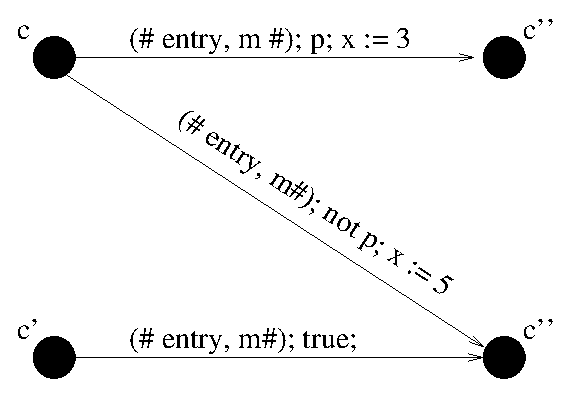
\epsfig{file=annotgen_example, width=4cm}
\end{center}
\caption{MVA fragment to illustrate set-annotation
generation}\label{FigAnnotGenExample}

\end{figure}
\subsection{Step 1 of the Algorithm}
The annotation generation algorithm selects the appropriate class of a
program and annotates all relevant methods. The algorithm proceeds as
follows.
\begin{enumerate}
\item It is ensured that all methods that have to be annotated have a
body in this class. If a method is inherited from a superclass, a
dummy-body is generated that directly calls the method from the
superclass.
\item New ghost variable declarations are added that encode the
control points of the automaton:
\begin{itemize}
\item for each control point of the automaton, a (final) ghost
variable declaration is generated, initialised to a unique value;
\item a ghost variable \texttt{cp} is declared, initialised to the
value of the ghost variable representing the initial control point;
\item for each automaton variable declaration, a ghost variable is
declared with corresponding type and initialisation.
\end{itemize}
\item A class invariant is added that the ghost variable \texttt{cp}
should never be equal to the value of the ghost variable representing
the special control point \halted.
\item For each method that is mentioned in the set of events of the
MVA, appropriate pre-, post- and exceptional post-set annotations are
generated. The set annotations use the \CaseJML statement. The exact
algorithm is best illustrated with an example. Suppose that we have
the MVA displayed in Figure~\ref{FigAnnotGenExample}, where \texttt{x}
is supposed to be an automaton variable. It has 
three transitions labelled \(\opri \etype := \entry,
\mname := m\clri\) for some method \(m\). The \preset annotation
of method \(m\) contains a \CaseJML statement with three branches: the
first branch tests whether \texttt{cp} has the value of the ghost
variable representing control point \(c\) and \(p\) holds, the second
tests whether we are in \(c\) and \(\neg p\) holds \emph{etc.}. Notice
that the guards are now legal JML expressions, as all MVA variables
have been mapped into ghost variable declarations. In the first branch
\texttt{cp} is set to the ghost variable representing
\(c''\), and the ghost variable \texttt{x} is set to 3. In the second
branch,  \texttt{cp} is set to \(c'''\) and \texttt{x} to 5, and in
the last branch (\texttt{cp} = \(c'\)) \texttt{cp} is always set to
\(c'''\) and \texttt{x} is not changed.

Notice that the order in which the different cases are generated is
not important: since the MVA is total there is always exactly one case
that applies.
\end{enumerate}


\subsection{Step 2 of the Algorithm}
Once the set-annotations at method specification level are generated,
the next step is to translate further into legal JML
specifications. To ensure that the appropriate set-statements are
executed at the end of the method body, the body is wrapped in a
try-catch statement. The translation proceeds as follows.
\begin{enumerate}
\item The \CaseJML statements are translated into a sequence of \Set
statements; one for each ghost variable that is being assigned
somewhere in the \CaseJML statement. The expression that is being
assigned is a conditional expression, covering exactly all the
branches that update the variable, plus a default case that leaves the
variable unchanged.
\item The transformed \preset annotation is inserted before the first
line of the method body.
\item A special boolean ghost variable \texttt{ex} is declared. This
will be used to flag exceptional termination.
\item The method body (including the set annotations preceding it) is
wrapped in a try-catch-finally statement. In the catch block, the
exceptional post set-annotation is added, the flag \texttt{ex} is set
to true and the exception is rethrown. In the finally block the value
of \texttt{ex} is tested. If \texttt{ex} is false, the post
set-annotations are executed. Finally, the flag \texttt{ex} is set to
false.  
\end{enumerate}



\subsection{Correctness}

The complete algorithm has been formalised in
PVS~\cite{OwreRRSS96}. Also, correctness of the algorithm has been
proven using the PVS theorem prover. The verification of the two steps
of the algorithm have been done independently. To show correctness of
the algorithm, we prove the following:
\begin{enumerate}
\item Let program \(P\) be monitored by MVA \(a\). Suppose monitoring never
reaches the special state \(\halted\), and moreover runtime checking
of program \(P\) does not throw any \JMLExc. Let \(AP\) be the
resulting program of the first step of the annotation generation
algorithm applied to \(P\) and \(a\). Then runtime checking of \(AP\)
will not throw any \JMLExc.
\item Let \(P\) be an annotated program. If we apply any of the
transformations described in step 2 of the annotation generation
algorith, the behaviour of the program does not change.
\end{enumerate}
In order to prove these statements, we use the following auxiliary results.
